\documentclass[14pt]{extbook}
\usepackage{multicol, enumerate, enumitem, hyperref, color, soul, setspace, parskip, fancyhdr} %General Packages
\usepackage{amssymb, amsthm, amsmath, bbm, latexsym, units, mathtools} %Math Packages
\everymath{\displaystyle} %All math in Display Style
% Packages with additional options
\usepackage[headsep=0.5cm,headheight=12pt, left=1 in,right= 1 in,top= 1 in,bottom= 1 in]{geometry}
\usepackage[usenames,dvipsnames]{xcolor}
\usepackage{dashrule}  % Package to use the command below to create lines between items
\newcommand{\litem}[1]{\item#1\hspace*{-1cm}\rule{\textwidth}{0.4pt}}
\pagestyle{fancy}
\lhead{Progress Quiz 1}
\chead{}
\rhead{Version C}
\lfoot{1269-8776}
\cfoot{}
\rfoot{Fall 2020}
\begin{document}

\begin{enumerate}
\litem{
Write the equation of the line in the graph below in Standard form $Ax+By=C$. Then, choose the intervals that contain $A, B, \text{ and } C$.
\begin{center}
    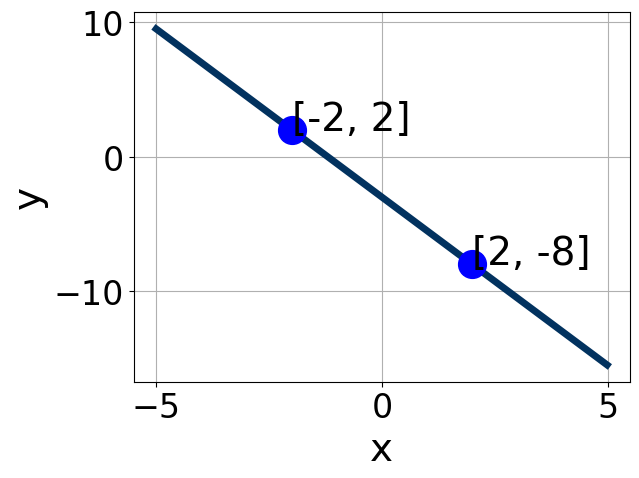
\includegraphics[width=0.5\textwidth]{../Figures/linearGraphToStandardC.png}
\end{center}
\begin{enumerate}[label=\Alph*.]
\item \( A \in [-4.4, -0.9], \hspace{3mm} B \in [4.16, 5.59], \text{ and } \hspace{3mm} C \in [2.8, 6.5] \)
\item \( A \in [-0.4, 5.4], \hspace{3mm} B \in [-5.9, -3.25], \text{ and } \hspace{3mm} C \in [-8, -1.5] \)
\item \( A \in [-2.4, 2.5], \hspace{3mm} B \in [0.46, 2.4], \text{ and } \hspace{3mm} C \in [-0.9, 2.3] \)
\item \( A \in [-2.4, 2.5], \hspace{3mm} B \in [-1.86, -0.55], \text{ and } \hspace{3mm} C \in [-1.9, 0.1] \)
\item \( A \in [-0.4, 5.4], \hspace{3mm} B \in [4.16, 5.59], \text{ and } \hspace{3mm} C \in [2.8, 6.5] \)

\end{enumerate} }
\litem{
Find the equation of the line described below. Write the linear equation as $ y=mx+b $ and choose the intervals that contain $m$ and $b$.\[ \text{Perpendicular to } 5 x - 9 y = 10 \text{ and passing through the point } (-4, -9). \]\begin{enumerate}[label=\Alph*.]
\item \( m \in [-2.8, -0.8] \hspace*{3mm} b \in [14.2, 17.2] \)
\item \( m \in [-2.8, -0.8] \hspace*{3mm} b \in [-5, -4] \)
\item \( m \in [-1.56, 0.44] \hspace*{3mm} b \in [-20.2, -10.2] \)
\item \( m \in [-2.8, -0.8] \hspace*{3mm} b \in [-20.2, -10.2] \)
\item \( m \in [1.8, 2.8] \hspace*{3mm} b \in [-1.8, 3.2] \)

\end{enumerate} }
\litem{
First, find the equation of the line containing the two points below. Then, write the equation as $ y=mx+b $ and choose the intervals that contain $m$ and $b$.\[ (-4, 9) \text{ and } (-5, -9) \]\begin{enumerate}[label=\Alph*.]
\item \( m \in [-18, -16] \hspace*{3mm} b \in [-105, -95] \)
\item \( m \in [13, 19] \hspace*{3mm} b \in [-82, -75] \)
\item \( m \in [13, 19] \hspace*{3mm} b \in [-6, 2] \)
\item \( m \in [13, 19] \hspace*{3mm} b \in [76, 87] \)
\item \( m \in [13, 19] \hspace*{3mm} b \in [10, 14] \)

\end{enumerate} }
\litem{
Solve the equation below. Then, choose the interval that contains the solution.\[ -7(8x -16) = -9(6x + 17) \]\begin{enumerate}[label=\Alph*.]
\item \( x \in [0.7, 1.53] \)
\item \( x \in [-3.75, -3.31] \)
\item \( x \in [-2.27, -1.45] \)
\item \( x \in [-1.38, -0.04] \)
\item \( \text{There are no real solutions.} \)

\end{enumerate} }
\litem{
\begin{enumerate}[label=\Alph*.]

\end{enumerate} }
\litem{
Solve the linear equation below. Then, choose the interval that contains the solution.\[ \frac{-7x -3}{5} - \frac{3x -5}{4} = \frac{-4x + 3}{2} \]\begin{enumerate}[label=\Alph*.]
\item \( x \in [-1.26, -0.04] \)
\item \( x \in [-6.69, -6.22] \)
\item \( x \in [-22.62, -21.59] \)
\item \( x \in [-5.85, -5.61] \)
\item \( \text{There are no real solutions.} \)

\end{enumerate} }
\end{enumerate}

\end{document}